\section{Experimental setup}
    This exercise requires a Stokes' viscosity measurement device (see Figure \ref{apparatus}) with castor oil and some small metal balls. The experiment also requires devices including micrometer, calliper, densimeter, electronic scales, stopwatch, and thermometer.
    \begin{figure}[htbp]
        \centering
        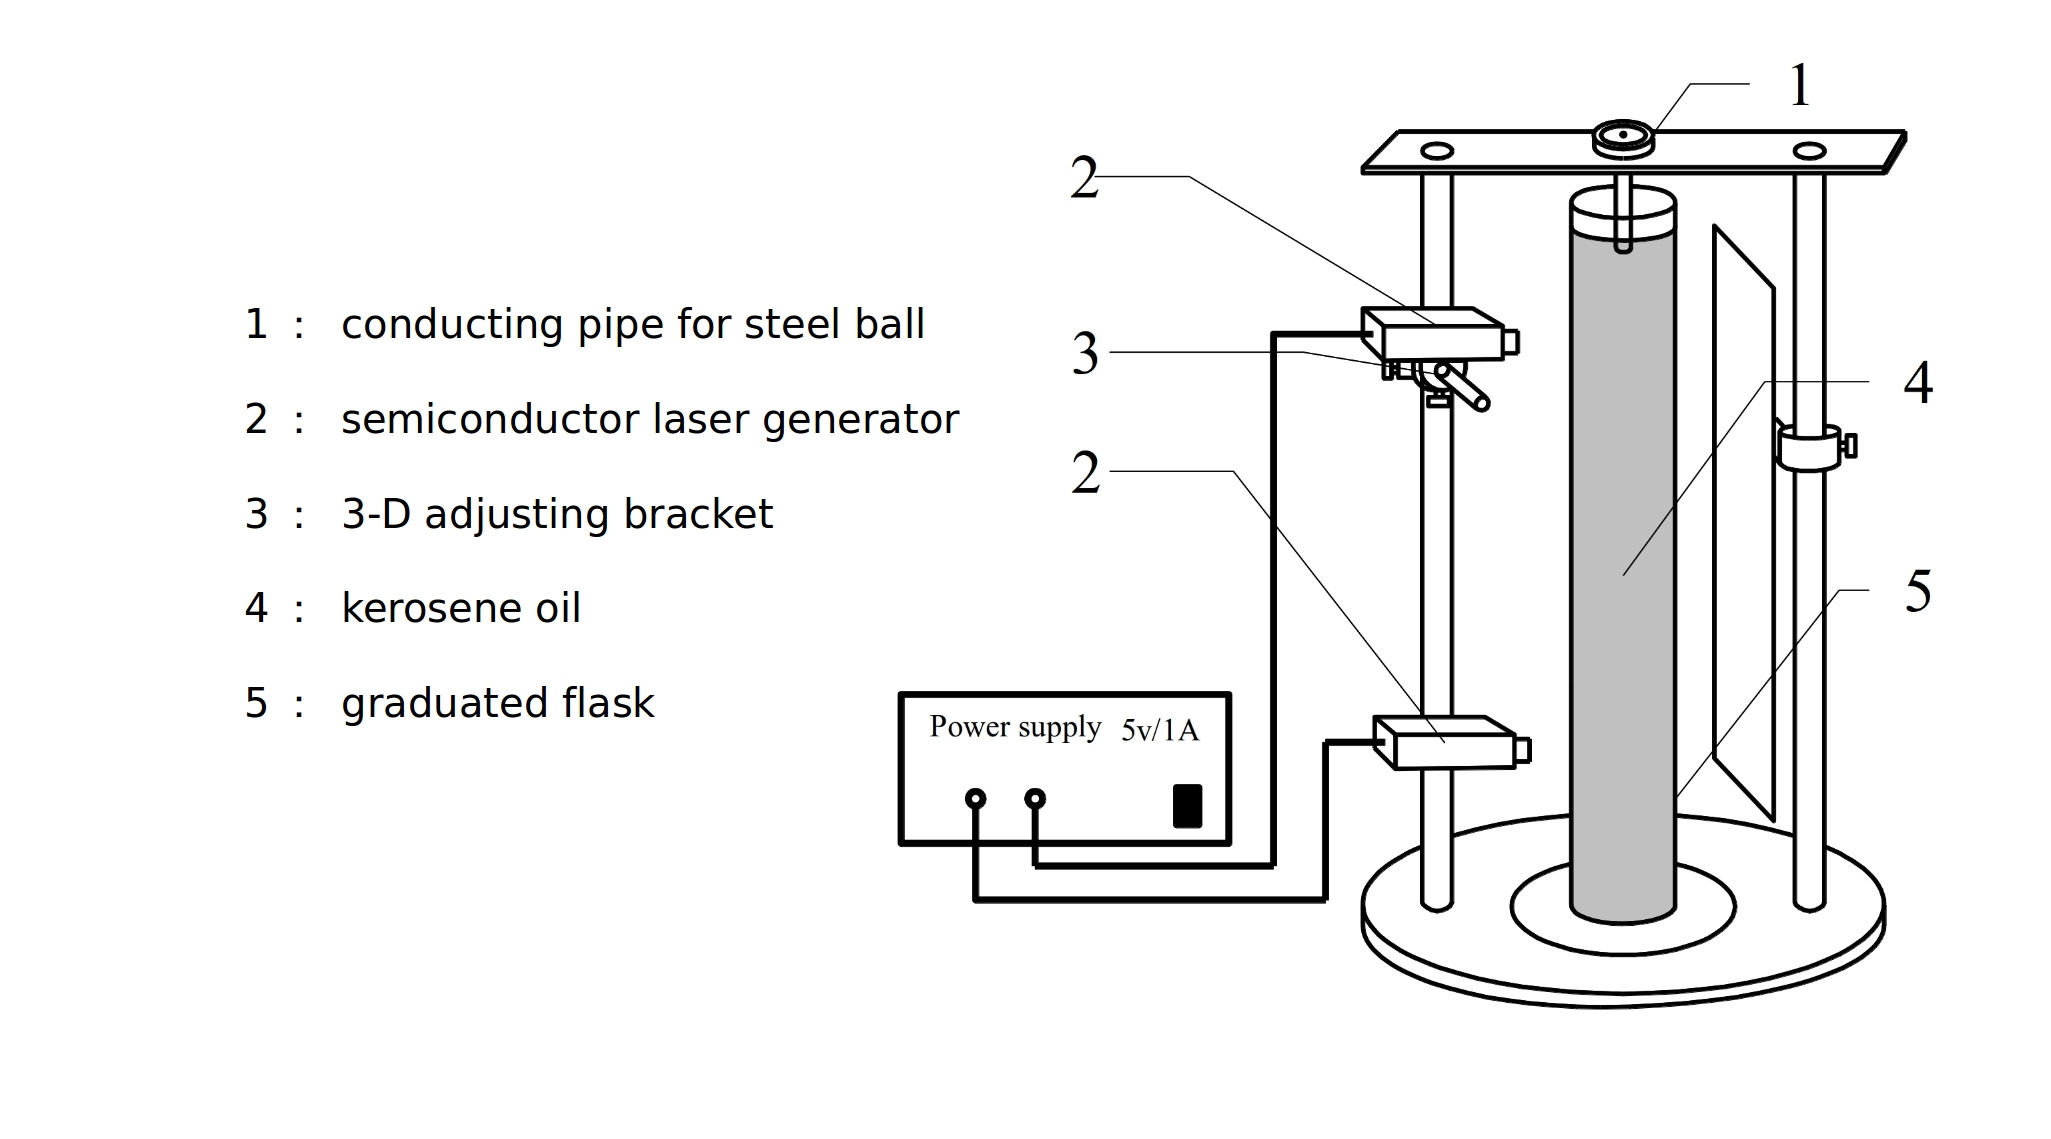
\includegraphics[width=0.8\linewidth]{images/1.png}
        \caption{Stokes’ viscosity measurement apparatus}
        \label{apparatus}
    \end{figure}

    The micrometer is used to measure the diameters of the balls, allowing measurements with maximum uncertainty of $0.004mm$. The calliper is used to measure the inner diameter of the flask, whose maximum uncertainty is $0.02mm$.The densimeter's maximum uncertainty is $0.001 g/cm^3$. The electronic scales' maximum uncertainty is $0.001g$. The stopwatch's maximum uncertainty is $0.01s$. The thermometer's maximum uncertainty is $\SI{2}{\degreeCelsius}$.\\